\documentclass{article}
\usepackage{amsmath}
\usepackage{tikz}
\usetikzlibrary{arrows.meta}

\begin{document}

\begin{figure}[h]
    \centering
    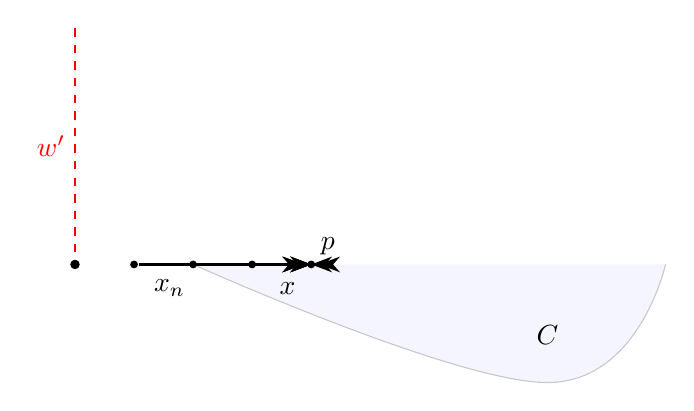
\begin{tikzpicture}[scale=1.5,auto=left]
        % Define styles
        \tikzset{
            mydot/.style={circle, fill, inner sep=1pt},
            myarrow/.style={-Stealth, line width=1pt}
        }
        
        % Draw the cone C
        \draw[opacity=0.2, fill=blue!20] plot [smooth, tension=.7] coordinates {(0,0) (3,-1) (4,0)};
        \node at (3,-0.6) {$C$};
        
        % Draw the support vector w'
        \draw[dashed, red] (-1,2) -- node[left, pos=0.5] {$w'$} (-1,0);
        \filldraw[black] (-1,0) circle (1pt);
        
        % Draw the sequence of support vectors (p_n)
        \node[mydot] (A) at (-0.5,0) {};
        \node[mydot] (B) at (0,0) {};
        \node[mydot] (C) at (0.5,0) {};
        \node[mydot] (D) at (1,0) {};
        
        \draw[myarrow] (A) -- (1,0);
        \draw[myarrow] (B) -- (1,0);
        \draw[myarrow] (C) -- (1,0);
        \draw[myarrow] (D) -- (1,0);
        
        % Draw the point x and its projection
        \node at (0.8,-0.2) {$x$};
        \node at (-0.2,-0.2) {$x_n$};
        \draw[myarrow, shorten >= 1mm, shorten <= 1mm] (A) -- (1,0);
        \draw[myarrow, shorten >= 1mm, shorten <= 1mm] (B) -- (1,0);
        \draw[myarrow, shorten >= 1mm, shorten <= 1mm] (C) -- (1,0);
        \draw[myarrow, shorten >= 1mm, shorten <= 1mm] (D) -- (1,0);
        
        % Label the limit point p
        \node[above right] at (1,0) {$p$};
    \end{tikzpicture}
    \caption{The vector \( w' \) describes the direction from which the sequence of support vectors \( (p_n)_{n \in \mathbb{N}} \) approaches the limit \( p \). Notice that the point \( x \) has the largest \( w' \)-component among all points on the corresponding face of \( C \).}
    \label{fig:cone_sequence}
\end{figure}

\end{document}